\documentclass[12pt, oneside]{article}   	                 		
\usepackage{graphicx}
\usepackage{epstopdf}
\usepackage{cite}
\usepackage{setspace}
\usepackage{mathtools}
\usepackage{amsmath}
\usepackage{caption}
\usepackage{subcaption}
\usepackage{tabularx}
\usepackage{fullpage}  
\usepackage{enumerate}
\usepackage{url} 
\usepackage{multicol}
\usepackage{appendix}
\usepackage[section]{placeins}
\usepackage{morefloats}
\usepackage{topcapt}
\usepackage{graphicx}
\graphicspath{{/home/wwwennie/wwwennie@gmail.com/UT-Austin/teaching/Elective-Computational-Methods-MatSci/projects/2-lattice-sums/figs/}}

\title{PSet 2: Lattice Sums, Part 1}
\author{Solutions}
\date{}

\begin{document}
\maketitle

Attached is the following code that was used in this problem set

\begin{enumerate}
    \item make\textunderscore latt.py: make FCC and BCC lattice
    \item lat\textunderscore sum.py: lattice sum routines, modifications 1-5
    \item PS2-*.py: code for generating plots corresponding to homework problems
\end{enumerate}

%--------------------------------------------------------------------------------%
\section{Exercise 1: Simulate lattice sum of FCC cell with Lennard-Jones Potential}

This is already implemented in the code given. Relevant lattice sum codes include are lat\textunderscore sum\# for \# = 1, 2, 3, 4, 5. 

 \begin{enumerate}
   \item lat\textunderscore sum1    $\rightarrow$ naive implementation of lattice sum with double counting
   \item lat\textunderscore sum2  $\rightarrow$ more efficient indexing without double counting
   \item lat\textunderscore sum3  $\rightarrow$ implementation with cutoff interaction
   \item lat\textunderscore sum4  $\rightarrow$ alternate with periodic boundary conditions
   \item lat\textunderscore sum5  $\rightarrow$ periodic boundary conditions using cutoff (e.g., for minimum image convention)
 \end{enumerate}
 
 Running these codes, one finds that all implementations of the lattice sums result in the same numerical answer. For small cells, the gain in efficiency is negligible. We use latsum5.m and assume the minimum image convention. 

%--------------------------------------------------------------------------------%
\section{Exercise 2: Equilibrium parameters for FCC}

To find the minimum equilibrium energy and lattice parameter, we vary the lattice parameter for a fixed cutoff energy. Figure \ref{fig:eqlattfcc} shows the energy calculated for a relatively small cell consisting of 3 repeating units in the three cartesian directions. For the purposes of these simulations, $\epsilon = \sigma = 1$. 

\begin{figure}[h]
   \centering
   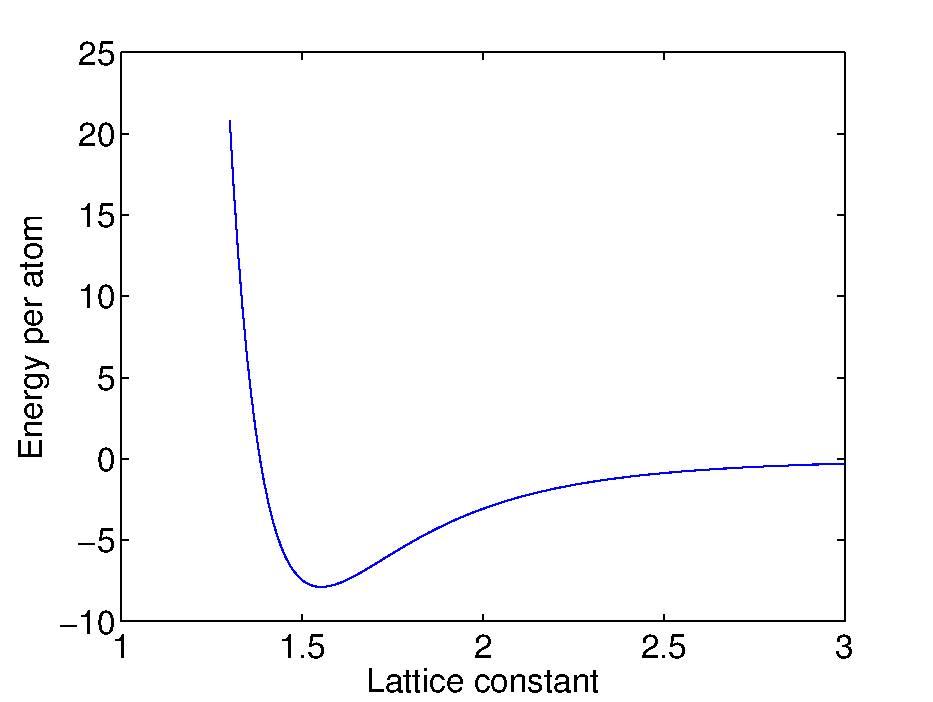
\includegraphics[width=0.7\textwidth]{eqlatt-fcc-n3} 
   \caption{Energy landscape as a function of lattice parameter for lattice sum of FCC lattice; n = 3 repeating units in each cartesian direction.}
   \label{fig:eqlattfcc}
\end{figure}

These parameters correspond to a 
minimum energy/atom: -7.8802 and 
equilibrium lattice constant: 1.553 


%--------------------------------------------------------------------------------%
\section{Exercise 3: Convergence with cutoff for FCC}

We test the accuracy of our choice of simulation by testing the radius cutoff used. The convention used is the minimum image convention with periodic boundary conditions, in which the cutoff distance is taken to be less than or equal to half the size of the simulation cell. For convenience, we take the cutoff distance to be half the size of simulation cell and modulate the size of the simulation cell. 

We plot the change in energy with respect to cutoff for a fixed lattice size. This is demonstrated in Figure \ref{fig:rcsfcc}, which plots the convergence of energy per atom with respect to the number of nearest neighbors. For the FCC lattice, the nearest neighbor distance is $\frac{a_0}{\sqrt{2}}$. The effective nearest neighbors taken into consideration for the interaction cutoff radius is found from the quotient of the cutoff with nearest neighbor distance.

\begin{figure}[h]
   \centering
   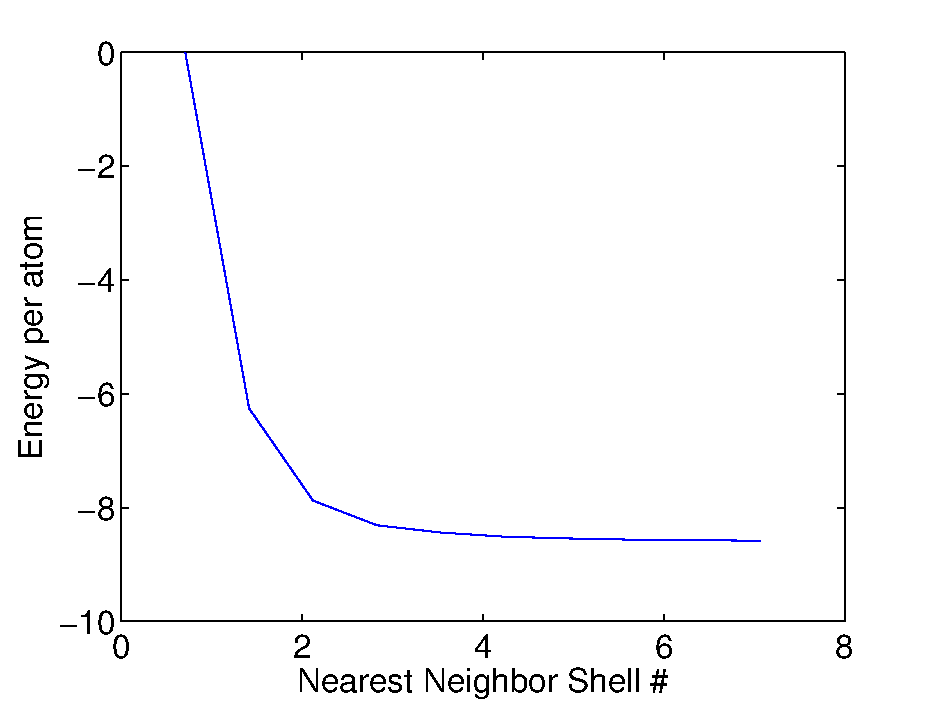
\includegraphics[width=0.8\textwidth]{rc-conv-fcc} % requires the graphicx package
   \caption{Convergence of energy per atom for LJ potential in FCC lattice with respect to nearest neighbor shells, using $a_0 = 1.55$}
   \label{fig:rcsfcc}
\end{figure}

As seen in Figure \ref{fig:rcsfcc}, it requires on the order of 5 repeating FCC unit cells (i.e., around 4 neighbor shells) to sufficiently begin to capture the long range interactions between all atoms, though larger simulation cells would be needed to capture the correct minimum energies.
 
 \begin{table}[htbp]
\centering
\caption{Convergence of lattice parameter and energy per atom for FCC atom using LJ potential; all cutoffs are half the simulation cell size;  $\infty$ cutoff is theoretical value}
\label{tab:fcconv}
	\begin{tabular}{llll}
	\hline \hline
                 Cutoff (rcs, in units of $a_0$) &  Equil. Lattice constant & Equil. Energy per atom  & $\Delta$Energy \\
                 \hline 
                    1	&  1.587	& -1.4999  	& ---	\\
                   1.5	&  1.553	& -7.8802   	& -6.3803	\\
                   2.5	&  1.544	& -8.4424   	& -0.5522	\\
                   3.5	&  1.543	& -8.5492   	& -0.1068	\\
                    5	&  1.542	& -8.5905   	& -0.0413	\\
                    6  &   1.542   &  -8.5980         & -0.0075 \\
	  \hline
	       $\infty$     & ---	& -8.6362 	& error $\approx$ -0.0382 	\\
	\hline \hline	
\end{tabular}
\end{table}

Table \ref{tab:fcconv} illustrates the numerical convergence of lattice parameter and energy per atom for different cutoffs. Though the equilibrium lattice constant converges quickly within tens of unit cells, simulations cells on the order of 150 unit cells are needed for proper convergence for the equilibrium energy. 

The infinite lattice sum for the FCC lattice has been computed, and is a useful reference for the error in interaction cutoff. In assuming $\epsilon = \sigma = 1$, the Lennard-Jones potential takes the form

\begin{equation} 
  U_{cell}(r) = 4((\frac{1}{r})^{12} - (\frac{1}{r})^6).
\end{equation} 

For an infinite lattice, the lattice sum comes to be 

\begin{equation} 
  u_{atom}(r) = \frac{U_(r)}{N_{atom}}= 2(A_{12}(\frac{1}{r_{nn}})^{12} - A_{6}(\frac{1}{r_{nn}})^6).
\end{equation} 

For an FCC lattice, $A_{12}$ = 12.1318 and $A_{6}$ = 14.4539. With the calculated equilibrium lattice constant $a_0 = 1.54 $ (i.e. $r_{nn} \approx 1.0903 $), $ u_{atom} \approx -8.6362 $. This is approximately an error of 0.0382 when compared to the largest cutoff tested; a larger simulation cell would be needed for better precision. 

%--------------------------------------------------------------------------------%
\section{Exercise 4: Comparison with BCC lattice}

We next simulate the LJ potential using the BCC lattice. A similar summary to the FCC lattice for the BCC lattice is presented below. 

For 3 repeated unit cells in the three cartesian directions, we obtain a minimum energy of -6.8472 and corresponding equilibrium lattice constant of 1.253, as seen in Figure \ref{fig:eqlattbcc}.

It takes around 7 repeated units cells (i.e., 7 x 7 x 7 simulation cell) or around 4 nearest neighbor shells to begin to converge in energy.

\begin{figure}[h]
   \centering
   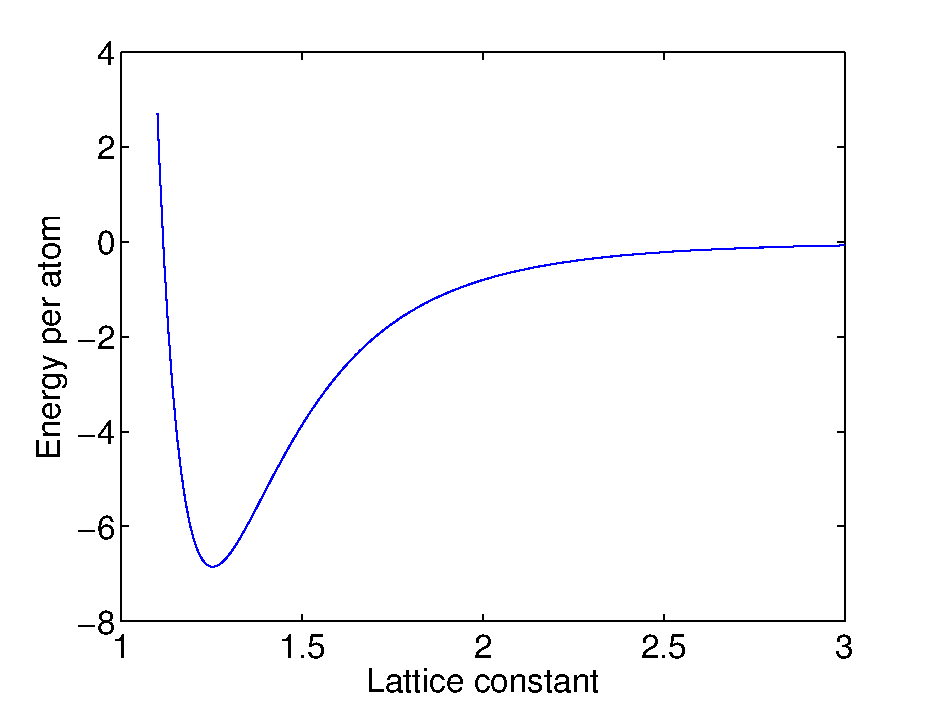
\includegraphics[width=0.7\textwidth]{eqlatt-bcc-n3} 
   \caption{Energy landscape as a function of lattice parameter for lattice sum of BCC lattice; n = 3 repeating units in each cartesian direction.}
   \label{fig:eqlattbcc}
\end{figure}

\begin{figure}[h]
   \centering
   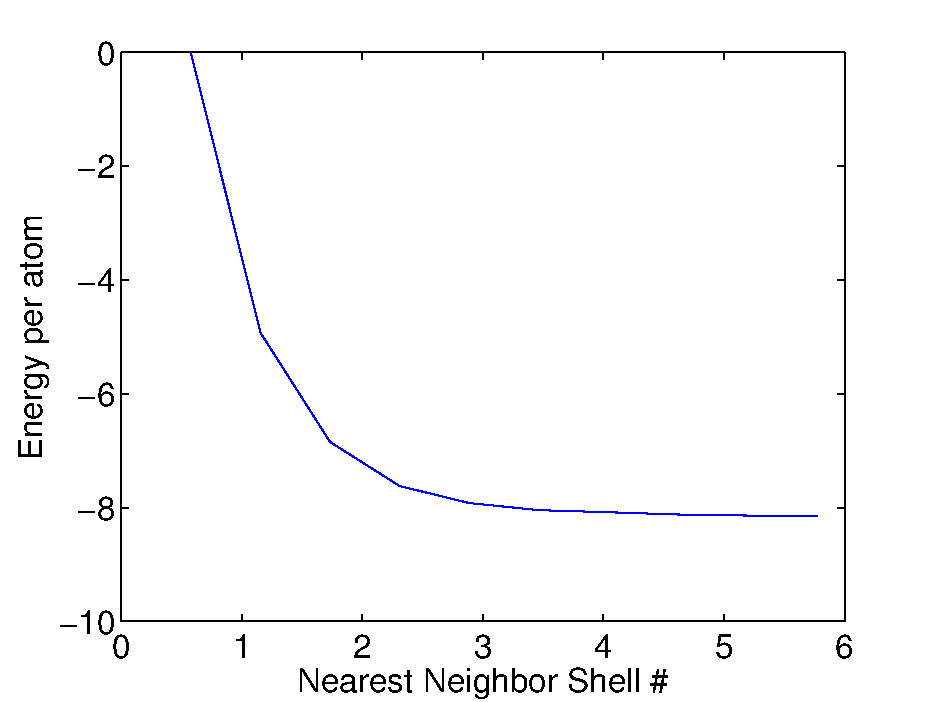
\includegraphics[width=0.8\textwidth]{rc-conv-bcc} % requires the graphicx package
   \caption{Convergence of energy per atom for LJ potential in BCC lattice with respect to nearest neighbor shells, using $a_0 = 1.25$}
   \label{fig:rcsbcc}
\end{figure}

 \begin{table}[htbp]
\centering
\caption{Convergence of lattice parameter and energy per atom for BCC atom using LJ potential; all cutoffs are half the simulation cell size; infinite cutoff is theoretical value}
\label{tab:bcconv}
	\begin{tabular}{llll}
	\hline \hline
                 Cutoff (rcs, in units of $a_0$) &  Equil. Lattice constant & Equil. Energy per atom  & $\Delta$Energy \\
                 \hline 
    		   1	&  1.296	&  -0.5000 	& ---	\\
                   1.5	&  1.253	&  -6.8472  	& -6.3472	\\
                   2.5	&  1.237	&  -7.9497  	& -1.1025	\\
                   3.5	&  1.235	&  -8.1212  	& -0.1715	\\
                    5	&  1.234	&  -8.1998   	& -0.0786	\\
	  \hline
	       $\infty$     & ---	&  -8.1896 	& error $\approx$ -0.0102 \\
          \hline \hline	
\end{tabular}
\end{table}


As the equilibrium energy for BCC more positive than that of FCC, it is less stable. 

For an infinite lattice, the lattice sum comes to be 

\begin{equation} 
  u_{atom}(r) = \frac{U_(r)}{N_{atom}}= 2(A_{12}(\frac{1}{r_{nn}})^{12} - A_{6}(\frac{1}{r_{nn}})^6).
\end{equation}  

For a BCC lattice, $A_{12}$ = 9.1142 and $A_{6}$ = 12.2533, $r_{nn} = \frac{\sqrt{3}a_0}{2} = 1.082 $, $ u_{atom} \approx -8.1896.$ This is corresponds to an error of 0.0102 for the largest simulation cell tested. Larger simulation cells are needed for better accuracies, but are not worth the time (at least without parallelization of some sort). 

%--------------------------------------------------------------------------------%
\section{Exercise 5: Thermodynamic parameters for FCC}

It is possible to calculate some thermodynamic quantities of relevance at 0K. At 0K (and constant temperature and volume), the Helmholtz free energy A is equivalent to the internal energy U. Thus, the pressure P

\begin{equation} 
  P = \frac{\partial A}{\partial V} \bigg|_{T,V}= \frac{\partial U}{\partial V}\bigg|_{T = 0K,V}.
\end{equation}  

\noindent Additionally, the Gibbs free energy is G = U + PV.

We plot the energy as a function of volume in Figure \ref{fig:evol}, which bears resemblance to the original Lennard-Jones potential. The volume as a function of pressure is subsequently shown in Figure \ref{fig:volp}, illustrating that with increasing pressure, the volume per unit cell is decreases; similarly, at no pressure, the simulation cell simply remains at its equilibrium volume. Figure \ref{fig:gibbsp} plots the Gibbs free energy as a function of pressure. 

\begin{figure}[htbp]
   \centering
   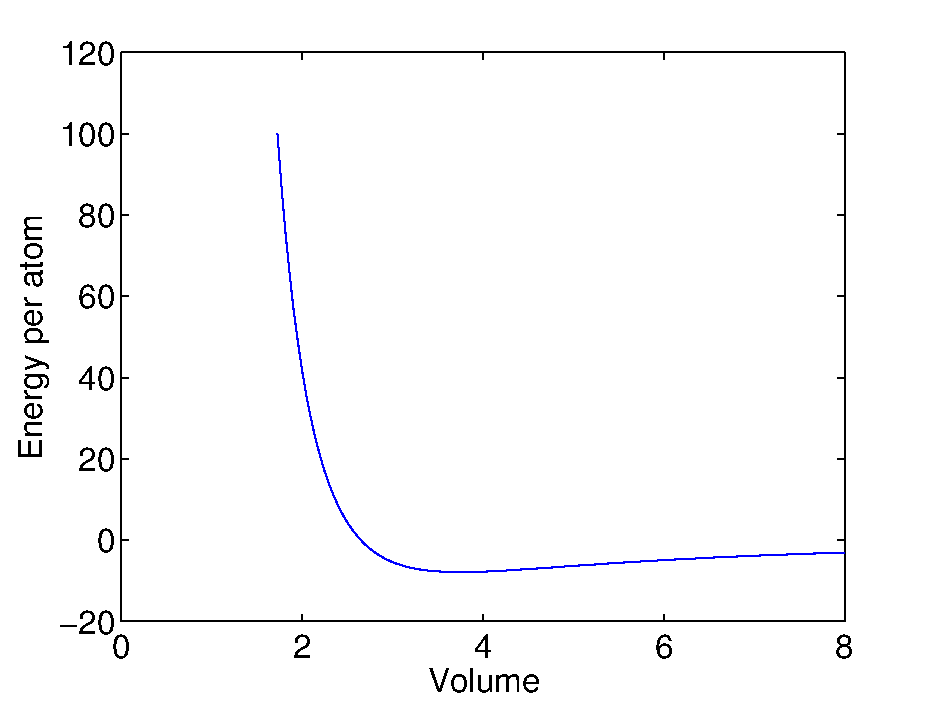
\includegraphics[width=0.7\linewidth]{e-vol} % requires the graphicx package
   \caption{Energy per atom versus volume of unit cell for 3 x 3 x 3 simulation supercell}
   \label{fig:evol}
\end{figure}

\begin{figure}[htbp]
   \centering
   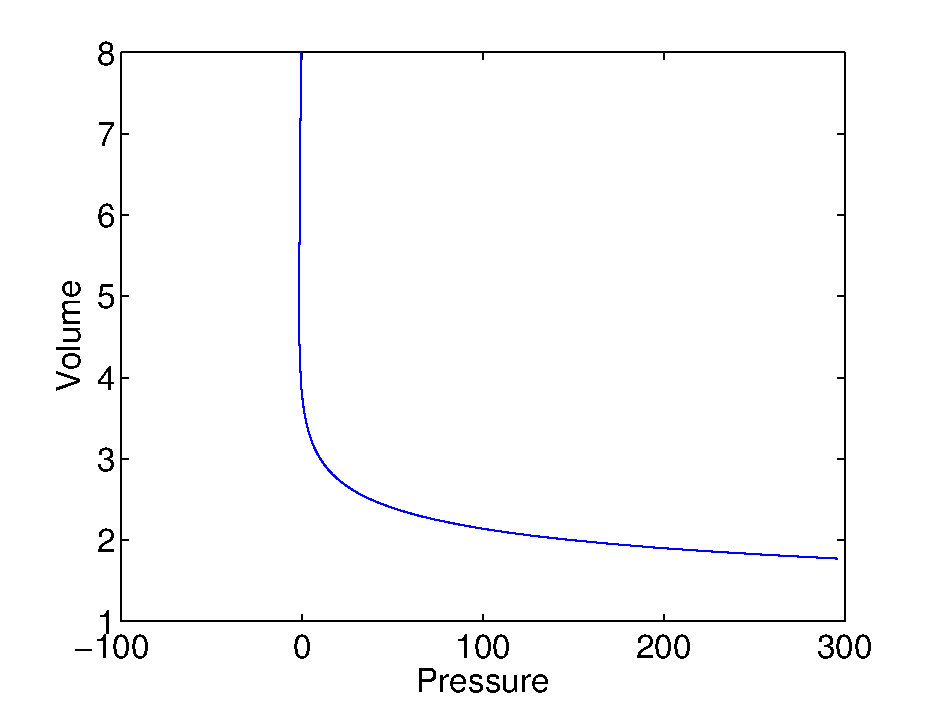
\includegraphics[width=0.7\linewidth]{vol-pressure} % requires the graphicx package
   \caption{Volume of unit cell versus pressure for 3 x 3 x 3 simulation supercell}
   \label{fig:volp}
\end{figure}

\begin{figure}[htbp]
   \centering
   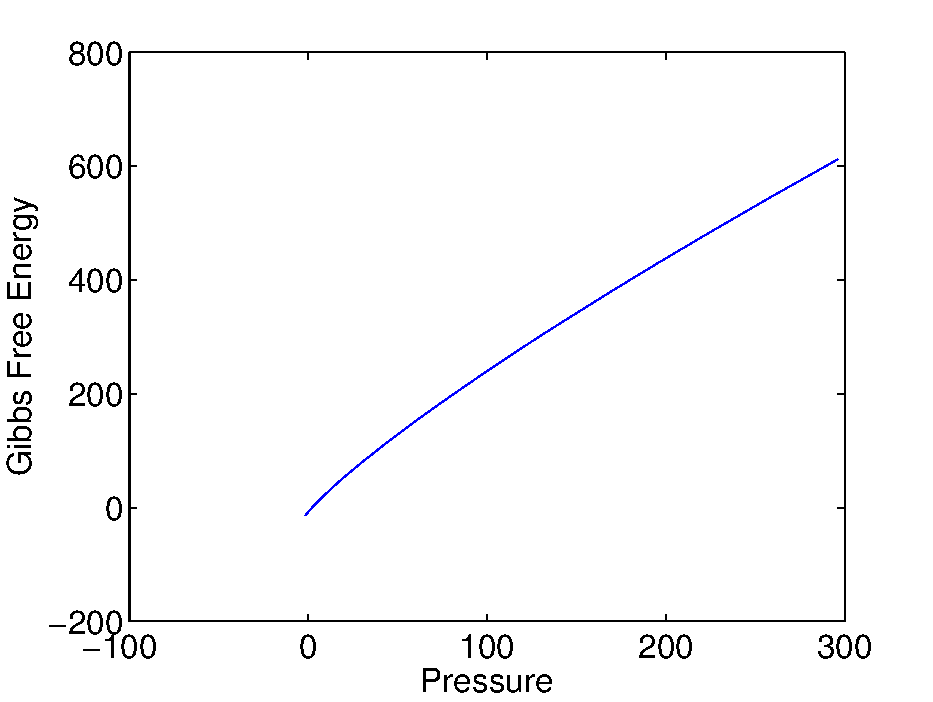
\includegraphics[width=0.7\linewidth]{gibbs-pressure} % requires the graphicx package
   \caption{Gibbs free energy versus pressure for 3 x 3 x 3 simulation supercell}
   \label{fig:gibbsp}
\end{figure}

\end{document}  

%% old tables %
% \begin{table}[htbp]
%\centering
%\caption{Convergence of lattice parameter and energy per atom for FCC atom using LJ potential}
%\label{tab:fcconv}
%	\begin{tabular}{llll}
%	\hline \hline
%                 Cutoff (rcs, in units of $a_0$) &  Equil. Lattice constant & Equil. Energy per atom  & $\Delta$Energy \\
%                 \hline 
%                2.5 	&  1.262	&  -1.2448 	& ---	\\
%                10 	&  1.254	&   -1.6505 	& 0.4057	\\
%                20 	&  1.253	&   -1.7186 	& 0.0681	\\
%                35 	&  1.252	&   -1.7478 	& 0.0292	\\
%                50 	&  1.252	&   -1.7596 	& 0.0118	\\
%                100 	&  1.252	&   -1.7732 	& 0.0136	\\
%                150 	&  1.252	&   -1.7778 	& 0.0046	\\
%                250 	&  1.252	&   -1.7814 	& 0.0036	\\
%	\hline \hline	
%\end{tabular}
%\end{table}
%
% \begin{table}[htbp]
%\centering
%\caption{Convergence of lattice parameter and energy per atom for FCC atom using LJ potential}
%\label{tab:fcconv}
%	\begin{tabular}{llll}
%	\hline \hline
%                 Cutoff (rcs, in units of $a_0$) &  Equil. Lattice constant & Equil. Energy per atom  & $\Delta$Energy \\
%                 \hline 
%                2.5 	&  1.583	&  -1.6619 	& ---	\\
%                10 	&  1.573	&   -2.5805 	& -0.9186	\\
%                20 	&  1.572	&   -2.7199 	& -0.1394	\\
%                35 	&  1.571	&   -2.7797 	& -0.0598	\\
%                50 	&  1.571	&   -2.8036 	& -0.0239	\\
%                100 	&  1.571	&   -2.8315 	& -0.0279	\\
%                150 	&  1.571	&   -2.8408 	& -0.0093	\\
%                250 	&  1.571	&   -2.8482 	& -0.0074	\\
%	\hline \hline	
%\end{tabular}
%\end{table}